%%%%%%%%%%%%%%%%%%%%%%%%%%%%%%%%%%%%%%%%%%%%%%%%%%%%%%%%%%%%%%%%%%%%%%%%
\chapter{Evaluation}
\label{sec:results}
%%%%%%%%%%%%%%%%%%%%%%%%%%%%%%%%%%%%%%%%%%%%%%%%%%%%%%%%%%%%%%%%%%%%%%%%

In this chapter, Procurrently will be evaluated based on the scenarios and compared to existing tools.
Furthermore, limitations compared to other tools will be described.

\section{Evaluating Scenarios}
\label{sec:eval}

Procurrently was evaluated using the scenarios described in \autoref{sec:scenarios}.
These were tested on a real git repository containing 600 files. One of the files most commonly used in testing was app.js containing over 7000 characters or about 200 lines. The test was run on two MacBook Pros using an 802.11ac Wi-Fi connection.
The bootstrap server was run on one of the MacBooks. The IP for the bootstrap server was configured before starting the test using the VS Code settings menu. 

\subsection{Scenario 1}

The branches used in the test were "bug-hunt" and "buildsystem-test". On branch bug-hunt, the files /app.js (see \autoref{fig:1appjs_on_bughunt}) and /routes/account.js (see \autoref{fig:1account_on_bughunt}) were modified by inserting comments. The configured username was "Stefan Gussner". 
After that on branch "buildsystem-test" the files /app.js and /routes/index.js were modified by inserting comments. The configured username was "Michael".


\begin{figure}
    \centering
    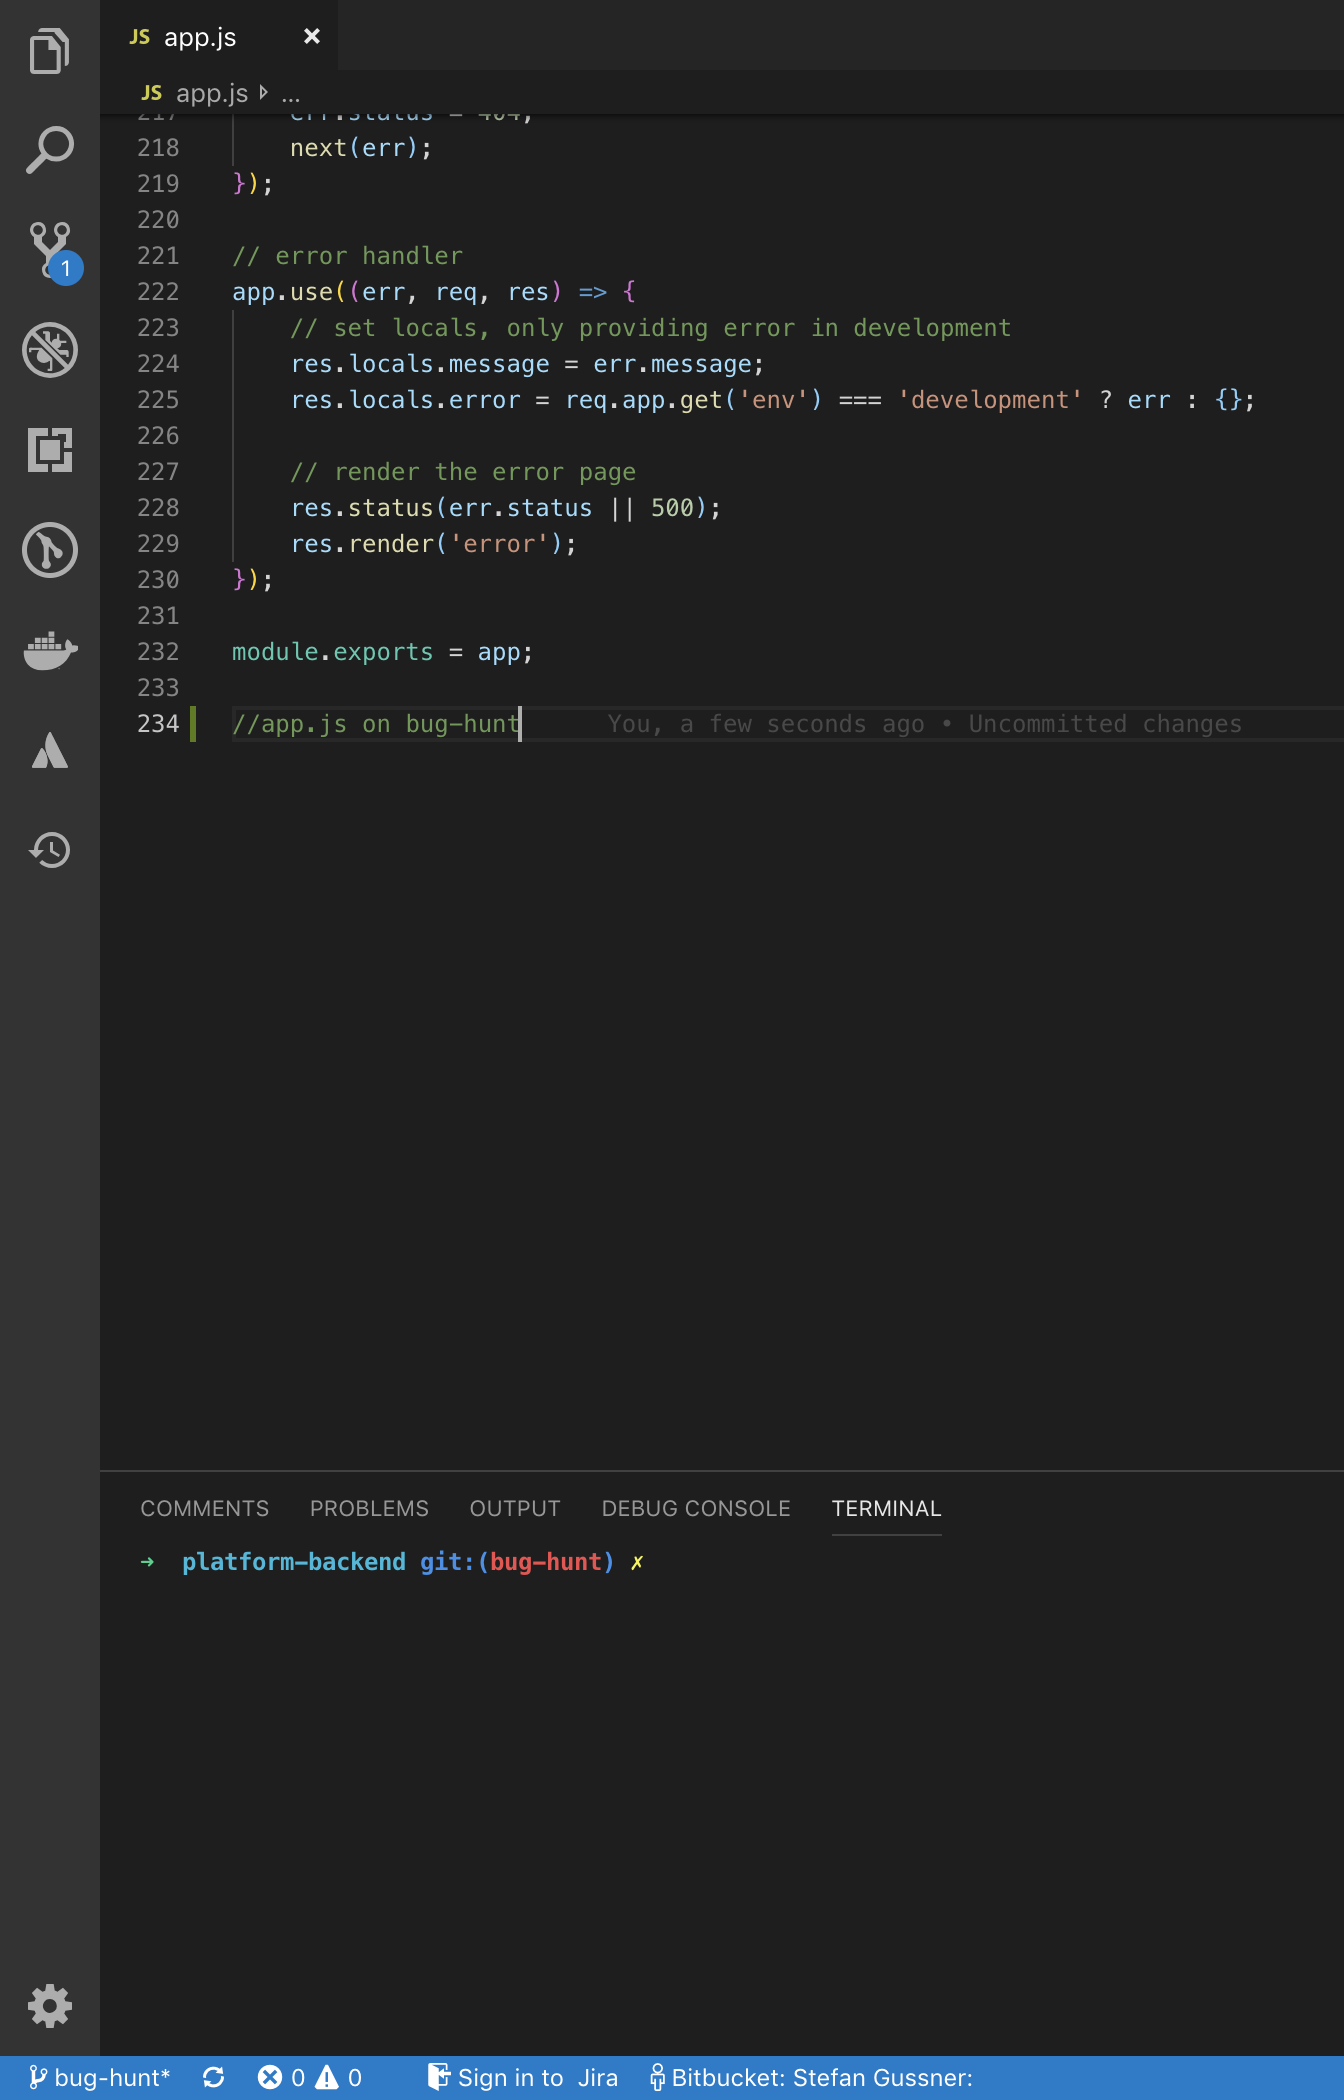
\includegraphics[width=1\linewidth]{figures/screenshots/scenarios/1appjs_on_bughunt.png}
    \caption{Scenario 1: Branch bug-hunt initial modifications app.js}
    \label{fig:1appjs_on_bughunt}
    \end{figure}
\begin{figure}
    \centering
    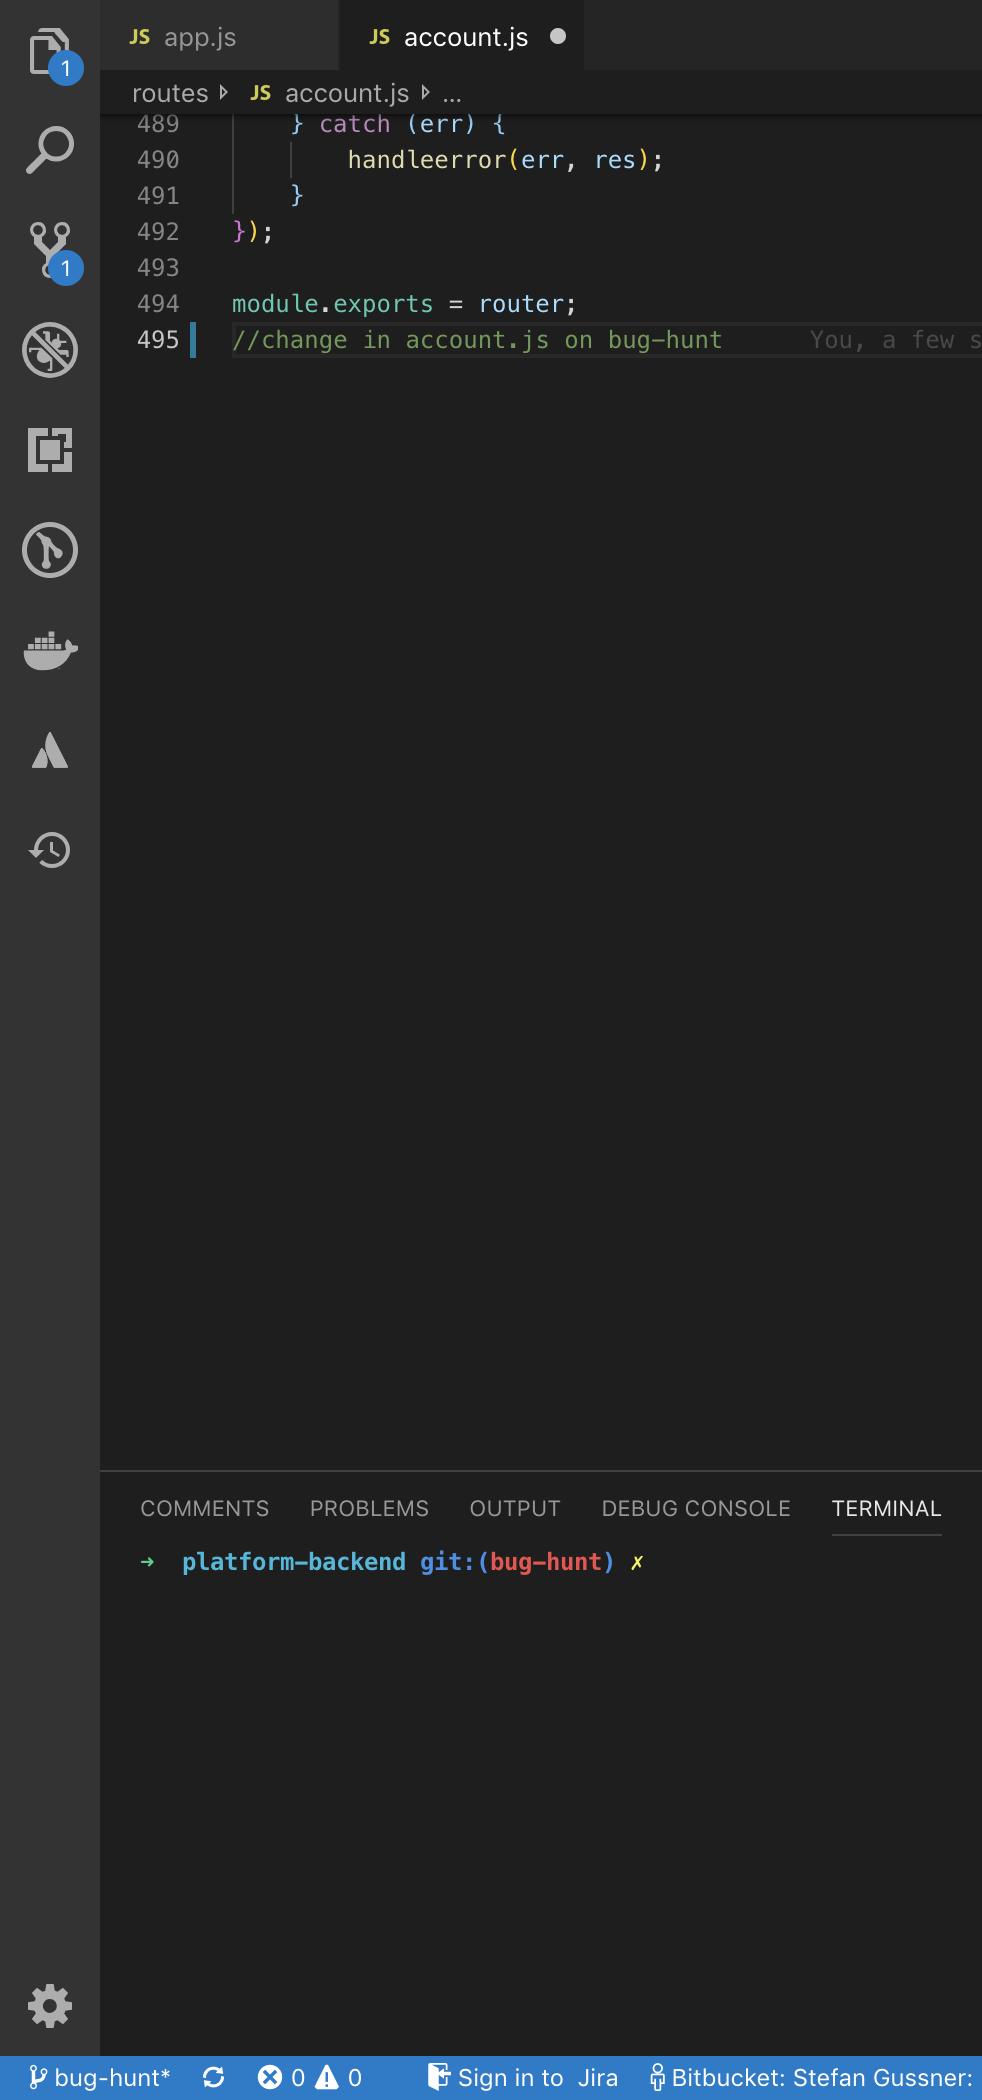
\includegraphics[width=1\linewidth]{figures/screenshots/scenarios/1accountjs_on_bughunt.png}
    \caption{Scenario 1: Branch bug-hunt initial modifications routes/account.js}
    \label{fig:1account_on_bughunt}
\end{figure}



\begin{figure}
    \centering
    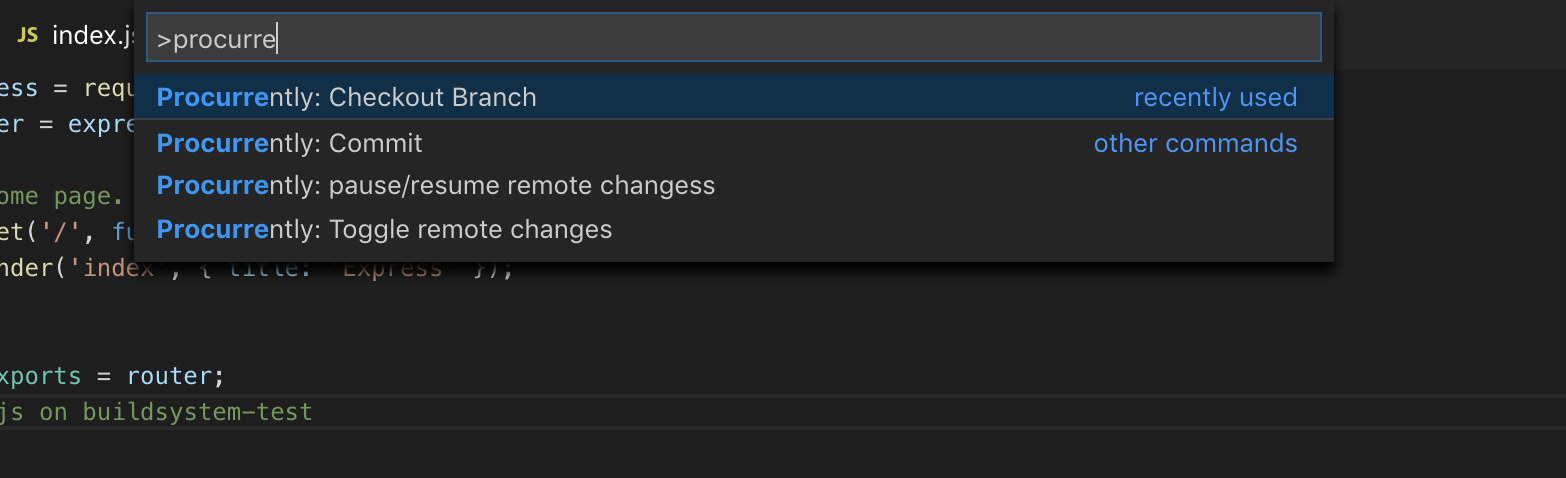
\includegraphics[width=1\linewidth]{figures/screenshots/scenarios/1checkout_branch.png}
    \caption{VS Code Command Palette Menu}
    \label{fig:1checkout_branch_palette}
\end{figure}
\begin{figure}
    \centering
    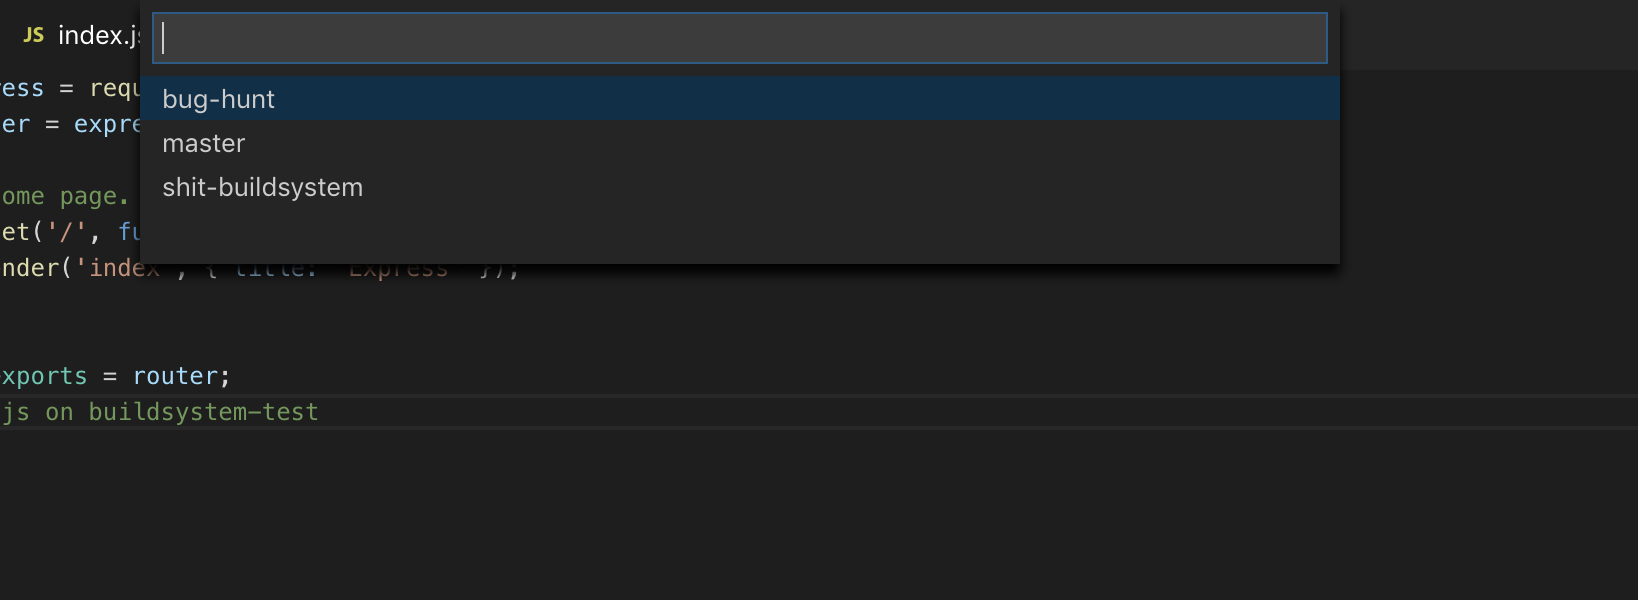
\includegraphics[width=1\linewidth]{figures/screenshots/scenarios/1checkout_bughunt.png}
    \caption{Select Branch}
    \label{fig:1checkout_bughunt}
\end{figure}


\begin{figure}[h]
    \centering
    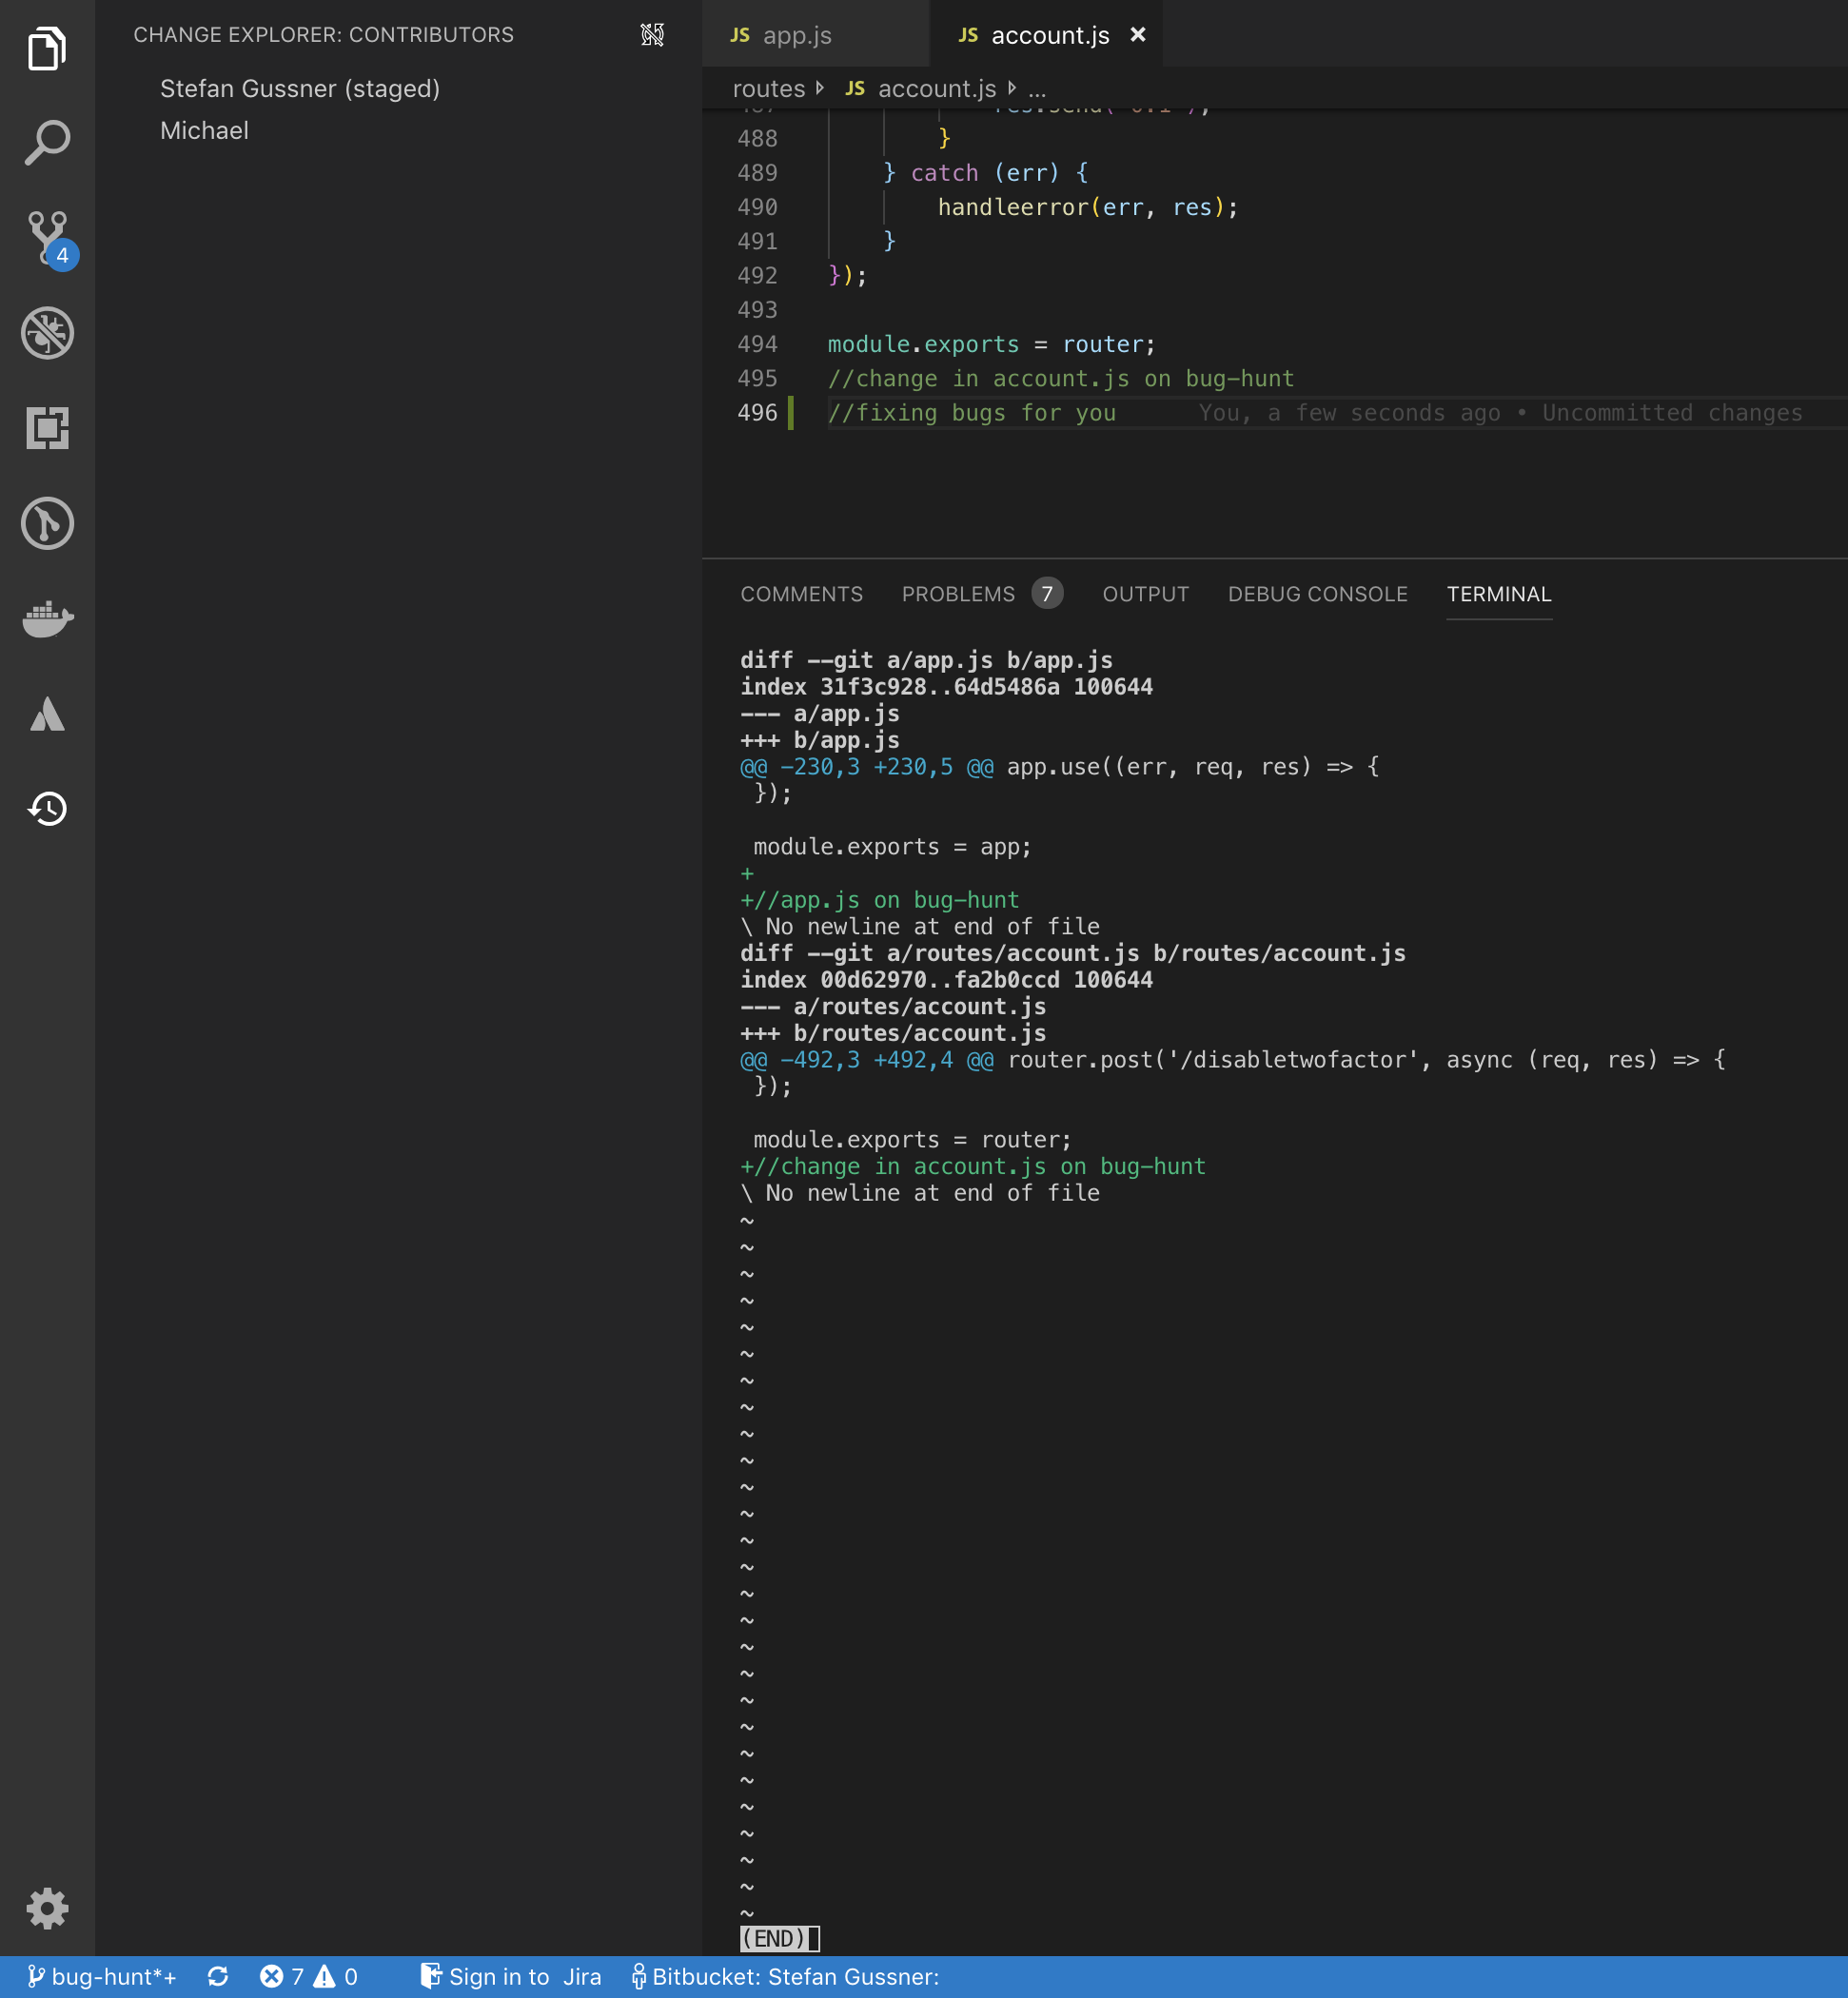
\includegraphics[width=1\textwidth]{figures/screenshots/scenarios/1staging_view.png}
    \caption{Scenario 1: account.js modified by Michael}
    \label{fig:1staging}
\end{figure}

On the computer with the Username "Michael" configured, the VS Code Command Palette was opened and the option Procurrently: Checkout Branch was selected (see \autoref{fig:1checkout_branch_palette}). From the presented options, the branch "bug-hunt" was selected (see \autoref{fig:1checkout_bughunt}). All the files were closed and the files /app.js and /routes/account.js were opened. The modifications on branch "bug-hunt" were visible in the files and the changes in branch "buildsystem-test" were no longer visible. The file /routes/account.js was modified by the computer with the Username "Michael" inserting another comment (see \autoref{fig:1staging}). The changes were immediately visible on the other computer. Using the VS Code Command Palette, the computer with the Username "Michael" configured switched back to branch "buildsystem-test".

\subsection{Scenario 2}

Both computers started out on the same branch. On the computer with the username "Stefan Gussner" a comment reading "comment from stefan" was created. On the other computer, a comment reading "comment from michael" was added (see \autoref{fig:2comments}). The VS Code Command Palette was used to execute the Procurrently: Toggle remote changes option (see \autoref{fig:2togglechanges}). After that, all remote changes were removed from the file, and only local changes were left (see \autoref{fig:2onlylocalchanges}). Later the Command Palette was used again to execute the Procurrently: Toggle remote changes command again to display the remote changes again.

\begin{figure}
    \centering
    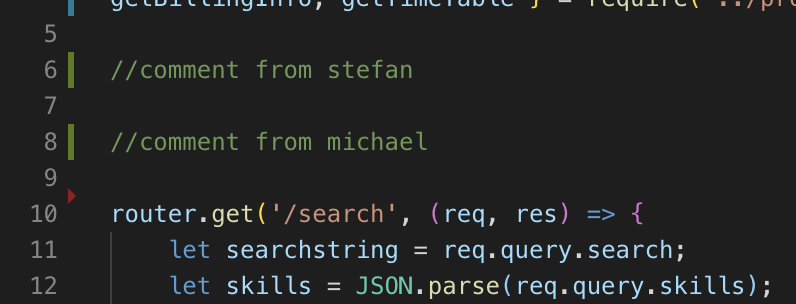
\includegraphics[width=1\textwidth]{figures/screenshots/scenarios/2comments.png}
    \caption{Scenario 2 - Comments Added by Both Collaborators}
    \label{fig:2comments}
\end{figure}
\begin{figure}
    \centering
    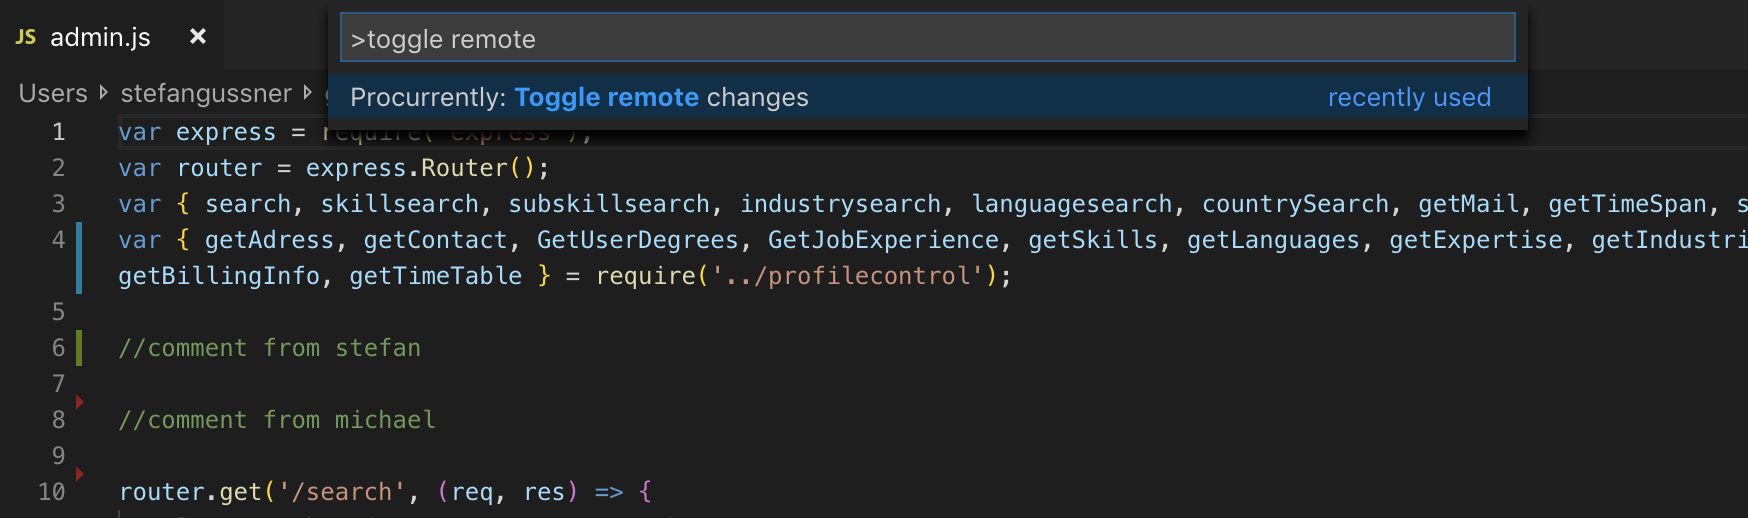
\includegraphics[width=1\linewidth]{figures/screenshots/scenarios/2togglechanges.png}
    \caption{Scenario 2 - VS Code Command Palette Menu Toggle Changes}
    \label{fig:2togglechanges}
\end{figure}

\begin{figure}[hb]
    \centering
    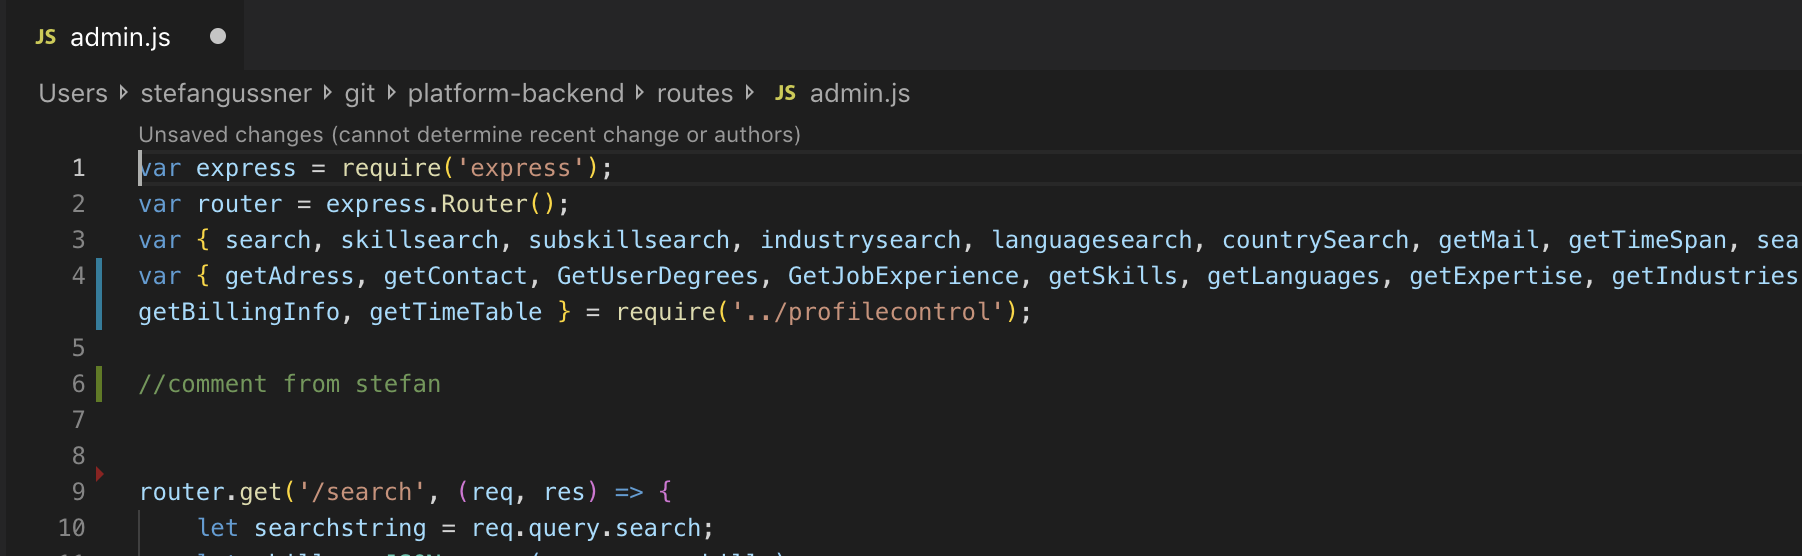
\includegraphics[width=1\textwidth]{figures/screenshots/scenarios/2onlylocalchanges.png}
	\caption{Scenario2: Only Local Changes Visible}
    \label{fig:2onlylocalchanges}
\end{figure}

\section{Results}
Procurrently succeeded in using the information provided by Git to provide branch-based real-time document synchronization. Only changes on the same branch are displayed to other users.

Changes to all documents in Git projects are shared with other peers (note that this is not the entire project structure as described in \autoref{limitations}).

Changes can be staged by author. This provides accountability and clarity about changes. \autoref{fig:stagebyauthor} shows staging a change by author using the Tree View panel. 

\begin{figure}[hb]
    \centering
    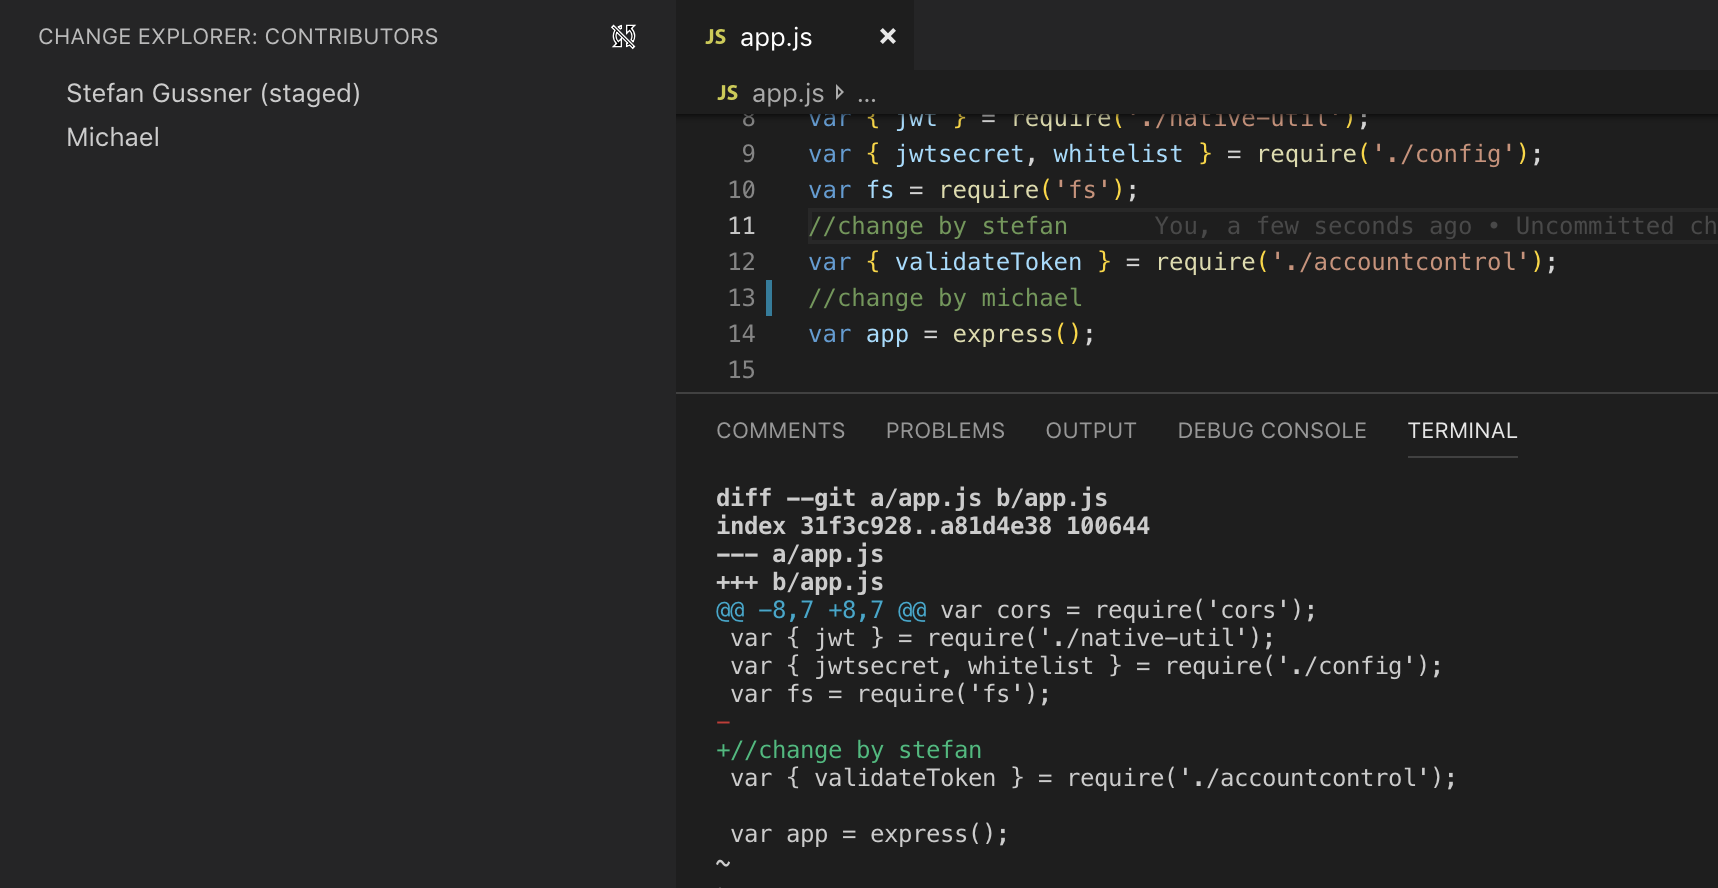
\includegraphics[width=150mm]{figures/screenshots/stage-by-author.png}
	\caption{Staging Changes by Author}
    \label{fig:stagebyauthor}
\end{figure}

Files defined to be ignored by Git are also ignored by Procurrently. This prevents accidentally publishing classified information and conflicts introduced by generated files. 

\subsection{Other Solutions}
Procurrently runs on the client and to some extent even works offline. Although some of the Tools described in \autoref{sec:stateoftheart} are client-side applications/extensions none of them provide support working offline. Having data available on the client at all times provides a performance advantage for Procurrently because when changesets have to be computed for displaying/hiding remote changes or branches are switched all the necessary data is already in memory on the device and is therefore very fast. It also enables real-time collaborations in environments without a stable internet connection such as trains.

Other solutions do not consider the version control system when providing real-time changes. This limits their usability in corporate environments. Procurrently is a tool for Git-based environments and their use cases in corporate environments. 

\subsection{Testing Procurrently in the Real-World}

Procurrently was tested in a real-world development environment with 2 users for 5 hours. After a short introduction to the new Git checkout procedure, the tool did not cause friction for the users. During the test situations similar to \autoref{sec:scenario1} were encountered multiple times. Procurrently was working as expected and aided the problem solution by providing fast context switching without the overhead of synchronizing changes via Git.

\section{Limitations}
\label{limitations}

Compared to other current solutions, Procurrently is unable to track files that do not exist in the last Git commit because the base version of a file is derived from the latest Git commit. This behaviour is necessary because some VS Code extensions create temporary files that do not get persisted to the filesystem but fire change events. Not ignoring these files would force developers to extend their .gitignore configuration and interfere with Procurrently's goal of not requiring extra configuration by the developer.

Procurrently is not secure. Anyone on the network can modify files in the repository. Also, all the traffic is unencrypted and can, therefore, be read by anyone on the network. This might not be a problem for open source projects as well as people working in corporate network environments.

The staging view does not differentiate between different branches, so all collaborators across all Git repositories and branches are presented as changes to be staged instead of filtering by collaborators who changed the current working context.

Due to the possible inconsistencies introduced by the asynchronous VS Code applyEdit API function and the workaround described in \autoref{subsec:concurrentchanges} processing huge change sets is noticeably slow. This is most obvious when processing multi cursor changes with more than 20 cursors at once.

Because the networking layer does not support UDP hole punching, a technique for traversing network address translation systems by sending udp packets, \cite{10.1007/978-3-642-20798-3_1} or similar techniques, communication between peers only works when clients are in the same local network.

Branch switching and committing changes sometimes have to be done through custom commands in VS Code instead of having the flexibility of doing those tasks using the command line and potentially using other programs or scripts to call those functions.

Procurrently enables switching branches while the current branch has been modified and the changes would be overwritten by Git. But this feature only works when using the custom VS Code command "Procurrently: Checkout Branch".

Procurrently's function to commit changes by an author only works properly if using the custom VS Code command "Procurrently: Commit". Otherwise, not committed changes will be lost after the commit because the changes are tied to the commit hash.

If there is no overlap between people working on a project, information about concurrent edits cannot be exchanged between peers.
One possible solution might be to host a Procurrently node in the Cloud. As described in \cite{6188603}, cloud-hosted nodes could be for Procurrently what GitHub is to Git. 
Peer to peer technology has been used to improve the Cloud before. \cite{Ranjan2013}, \cite{Ranjan2010}, \cite{Babaoglu:2012:DIP:2245276.2245357}. Cloud technology can be used to improve peer to peer software. This concept is used in the experimental Beaker Browser\footnote{https://beakerbrowser.com/docs/how-beaker-works/peer-to-peer-websites\#keeping-a-peer-to-peer-website-online}